% !TEX TS-program = pdflatex
% !TEX encoding = UTF-8 Unicode

% This is a simple template for a LaTeX document using the "article" class.
% See "book", "report", "letter" for other types of document.

\documentclass[11pt]{article} % use larger type; default would be 10pt

\usepackage[utf8]{inputenc} % set input encoding (not needed with XeLaTeX)

%%% PAGE DIMENSIONS
\usepackage{geometry} % to change the page dimensions
\geometry{a4paper} % or letterpaper (US) or a5paper or....

\usepackage{graphicx} % support the \includegraphics command and options

\usepackage{amssymb}
\usepackage{amsmath}
%%% PACKAGES
\usepackage{booktabs} % for much better looking tables
\usepackage{array} % for better arrays (eg matrices) in maths
\usepackage{paralist} % very flexible & customisable lists (eg. enumerate/itemize, etc.)
\usepackage{verbatim} % adds environment for commenting out blocks of text & for better verbatim
\usepackage{subfig} % make it possible to include more than one captioned figure/table in a single float
% These packages are all incorporated in the memoir class to one degree or another...

%%% HEADERS & FOOTERS
\usepackage{fancyhdr} % This should be set AFTER setting up the page geometry
\pagestyle{fancy} % options: empty , plain , fancy
\renewcommand{\headrulewidth}{0pt} % customise the layout...
\lhead{}\chead{}\rhead{}
\lfoot{}\cfoot{\thepage}\rfoot{}

%%% SECTION TITLE APPEARANCE
\usepackage{sectsty}
\allsectionsfont{\sffamily\mdseries\upshape} % (See the fntguide.pdf for font help)
% (This matches ConTeXt defaults)

%%% ToC (table of contents) APPEARANCE
\usepackage[nottoc,notlof,notlot]{tocbibind} % Put the bibliography in the ToC
\usepackage[titles,subfigure]{tocloft} % Alter the style of the Table of Contents
\renewcommand{\cftsecfont}{\rmfamily\mdseries\upshape}
\renewcommand{\cftsecpagefont}{\rmfamily\mdseries\upshape} % No bold!
\usepackage{graphicx}
\graphicspath{ {./pings/} }

\usepackage{amsmath}
\DeclareMathOperator*{\argmax}{arg\,max}
\DeclareMathOperator*{\argmin}{arg\,min}

\newcount\colveccount
\newcommand*\colvec[1]{
        \global\colveccount#1
        \begin{pmatrix}
        \colvecnext
}
\def\colvecnext#1{
        #1
        \global\advance\colveccount-1
        \ifnum\colveccount>0
                \\
                \expandafter\colvecnext
        \else
                \end{pmatrix}
        \fi
}

%%% END Article customizations

%%% The "real" document content comes below...

\title{Macro PS5}
\author{Michael B. Nattinger\footnote{I worked on this assignment with my study group: Alex von Hafften, Andrew Smith, and Ryan Mather. I have also discussed problem(s) with Emily Case, Sarah Bass, and Danny Edgel.}}

%\date{} % Activate to display a given date or no date (if empty),
         % otherwise the current date is printed 

\begin{document}
\maketitle

\section{Question 1}
Working-age agents maximize their value subject to their budget constraint:
\begin{align*}
V_j(k) = \max_{k',l}\{ u^W_j(c,l) + \beta V_j(k_{t+1})\}
\text{s.t. } c = (1-\tau) w e l + (1+r)k - k' 
\end{align*}
We will take first order conditions to solve for $l$ as desired.
\begin{align*}
\frac{\partial V_j}{\partial l} &= 0\\ \Rightarrow (c^\gamma(1-l)^{1-\gamma})^{-\sigma}\left( \gamma c^{\gamma-1}\frac{\partial c}{\partial l}(1-l)^{1-\gamma} - c^{\gamma}(1-l)^{-\gamma}(1-\gamma)\right) &= 0 \\
\Rightarrow \gamma\left( \frac{1-l}{c}\right)^{1-\gamma}(1-\tau)w e &= \left( \frac{1-l}{c}\right)^{-\gamma}(1-\gamma) \\
\Rightarrow \frac{\gamma}{1-\gamma}(1-l)(1-\tau)we_j &= c = (1-\tau)we_jl + (1+r)k - k' \\
\Rightarrow \frac{\gamma}{1-\gamma}(1-\tau)we_j  &= \left(\frac{\gamma}{1-\gamma}+1\right)(1-\tau)we_jl + (1+r)k - k' \\
\Rightarrow \frac{\gamma}{1-\gamma}(1-\tau)we_j - [ (1+r)k - k'] &= \left(\frac{1}{1-\gamma}\right)(1-\tau)we_jl \\
\Rightarrow \frac{\gamma(1-\tau)we_j - (1-\gamma)[(1+r)k - k']}{(1-\tau)we_j} &=  l.
\end{align*}

\section{Question 2}
Completed Matlab code is supplied with this solution. Note that it automatically loops through the non-social security and social security versions.
\section{Question 3}
\begin{itemize}
\item
The outermost loop iterates the entire procedure until either the maximum number of iterations is achieved, or until the model has converged (i.e. updated (labor) capital is within the tolerance of the old (labor) capital).
\item
The next loop goes through each old agent generation, one at a time. It begins with the oldest generation and procedes backwards in age, one generation at a time.
\item 
The next for loop iterates through assets that the agent will be given to hold today.
\item
The next loop loops through the assets that the agent will consider to hold tomorrow. The loop calculates the value from each combination of assets held today and tomorrow. There is an if clause at the end of this loop that stores the current optimal choice of savings conditional on the level of initial capital for this generation, which is updated if the program finds a new, better combination.
\item Next, the program loops through the working households. it proceeds in a similar fashion, looping through possible asset combinations for today and tomorrow, calculating the value of each combination, and updating the optimal choice of saving for each initial capital level whenever it finds a combination that is better than the current best choice.
\item Next, the program calculates and stores the optimal capital savings level for each generation, by working forwards, one generation at a time, starting from the first generation and finding the optimal savings of each generation given the capital level they are given by the previous generation (the first generation starts with no capital). Then the code calculates the labor supplied by each working-age generation.
\item Outside of this loop, the program aggregates the labor supply and updates the guess on capital and labor demand according to the update rule (weighted average of old (labor, capital) guess and (labor, capital) supply implied by that guess).
\end{itemize}
\section{Question 4}

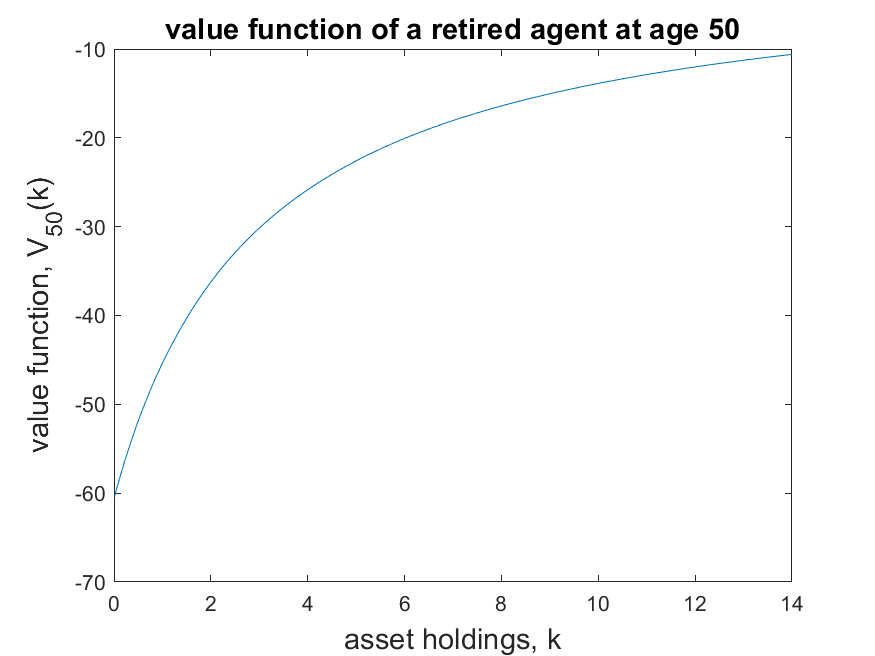
\includegraphics{fig1}

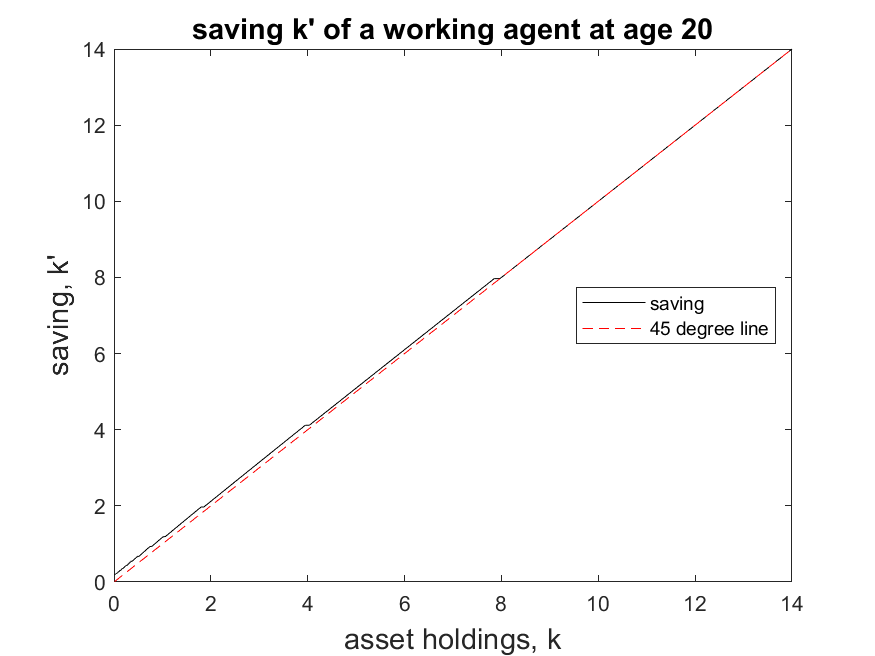
\includegraphics{fig2}

The value function over $k$ for a retired agent at $j=50$ is increasing and concave.  The savngs function for a worker at age $20$ is increasing in $k$, but the net savings $k'-k$ is decreasing in $k$.

\section{Question 5}

\subsection{Is the economy efficient?}
The interest rate (return on capital, $r=0.032$ without SS or $r=0.019$ with SS) is higher than the implicit return on social security (population growth rate, $n = 0.011$) so the economy is efficient.
\subsection{How does the economy compare with and without SS?}

The below table shows the difference in steady state values under social security and without.
\begin{center}
\begin{tabular}{lll}
& NoSS & SS \\ 
\hline 
kap & 3.9114 & 2.9777 \\ 
lab & 0.36866 & 0.351 \\ 
w & 1.4978 & 1.3819 \\ 
r & 0.019398 & 0.031622 \\ 
b & 0 & 0.21869 \\ 
V1 & -52.7642 & -54.6134 \\ 
W & -36.0338 & -35.0692 \\ 
\hline 
\end{tabular}
\end{center}

Capital increases as the agents must now save privately for retirement, rather than relying on the social security transfer. Labor increases a little bit without social security, as the workers no longer need to pay taxes on the wages they earn, and also because the higher capital increases the marginal productivity of labor.

\subsection{Wealth profiles by age group}

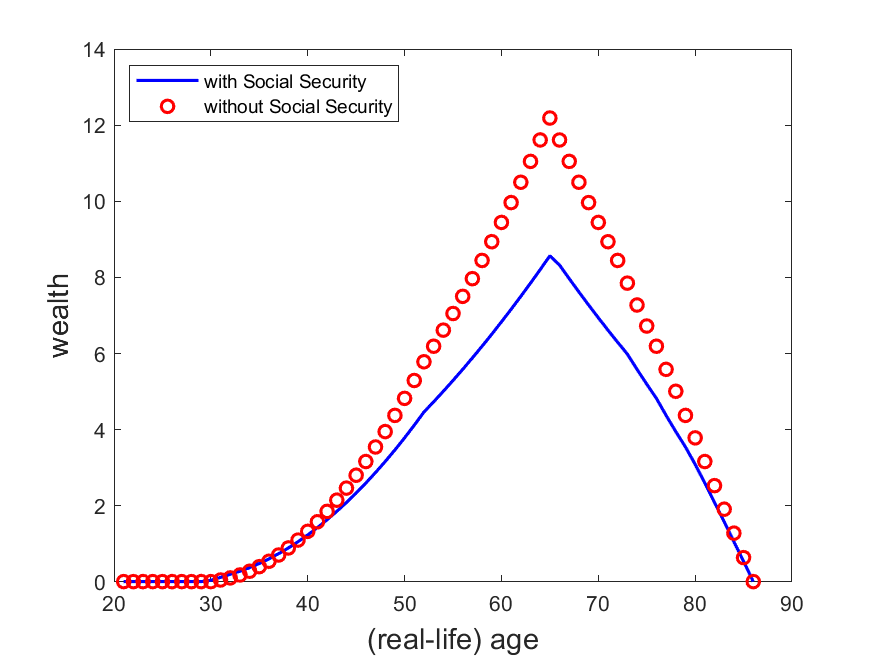
\includegraphics{fig3}

Without social security, the agents are incentivized to save more so they will have more wealth to live off of once they retire. As a result, the agents' net worth is higher throughout their lives.

\subsection{Newborn preference}
The newborn would prefer to be born in a world without social security, as the value in period 1 is $-52.76$ without social security, but only $-54.61$ with social security. The difference is because the agent is taxed in the first period under social security, but is does not recieve the benefit of the social security transfer until much later.

\subsection{Which is optimal overall?}
Aggregate welfare decreases by moving to the world without social security, to $-36.0$ without from $-35.1$ with social security. Thus, the majority of people would not vote for social security to be removed.
\end{document}
